\section{Creating the documentation}

\subsection{Collaboration and hosting}

Before scaffolding the actual project or picking tools that might help me putting the documentation together, I thought about where to host and how to enable collaborative content editing. The obvious choice for my purposes was \textit{GitHub}, as it solves numerous problems in an elegant and user-friendly way.

\begin{description}

	\item[Hosting]\hfill

	\textit{GitHub} provides a feature called \textit{GitHub Pages}. With the help of a specific \textit{Git} branch (\enquote{gh-pages}), all files on this branch (from the latest revision) can be accessed via \ac{HTTP} on port 80. This means that static \ac{HTML} files are served as websites to any browser. The service is free of charge, is based on a reliable server infrastructure and leverages \textit{GitHub's} \ac{CDN} for improved response times. Updating the content is as easy as committing changes to the \textit{gh-pages} branch and pushing them to the remote repository.

	By default, the website's address is \texttt{http(s)://\allowbreak\textbf{user-name}.github.io/\allowbreak\textbf{project-name}}. But \textit{GitHub} allows advanced \ac{DNS} settings, enabling the repository maintainer to point custom domains to the project page.

	\item[Collaboration]\hfill

	Each project has an issue tracker that allows \textit{GitHub} users to notify the repository maintainer about problems he discovered. These issues are public and everybody is free to join the discussion to propose solutions or suggestions.

	Taking this one step further, users can enrich issues by adding code (or textual content) that attempts to solve the problems they were facing. This procedure is then called a \textit{pull-request}. For the repository maintainer, applying the provided patches to the project is as easy as pushing a single button to confirm.

	To simplify the audition process of \textit{pull-requests} it is possible to integrate third-party \ac{CI} services that automatically compile and test proposed changes and then add the their results and logs to the issue discussion.

	\item[Content editor]\hfill

	Every directory and file of a repository that is hosted on \textit{GitHub} can be browsed on their website. In addition to that, files can also be edited with an online text editor which allows to quickly update content without cloning the repository. This is especially useful for text-based projects like documentations because it is not necessary to compile or test the project before submitting a patch.

	Another positive side effect of this approach, is that a user's edits automatically result in \textit{pull-request} which can then be easily audited and approved as described earlier.

	\item[Popularity]\hfill

	\textit{GitHub} is incredibly well-known and established among developers. Users tend to know the described collaboration workflows which lowers the barrier to actually bring oneself to participating.

\end{description}

\subsection{Static page generator}

Although the goal of the documentation is to only consist of static \ac{HTML} files, I intended to integrate a static page generator in order to optimize the development process. This leads to a build step, necessary to compile the source code to basic \ac{HTML} files before committing to \textit{gh-pages}. But that's a low price to pay, considering the indispensable advantages of this approach.

\begin{description}

	\item[Templating]\hfill

	With a static site generator it is possible to split a document into several files which may then be included as desired. This is especially useful to avoid code duplication considering that certain elements like a page header or footer have to be included into every page. It does also allow to split each section of a long article into separate files which makes it easier to find one's way around when editing content.

	\item[Dialects]\hfill

	It is possible to process languages that could not be interpreted by a browser. E.g. converting \textit{CoffeeScript} to \textit{JavaScript}, \ac{SASS} to \ac{CSS} or \textit{Markdown} to \ac{HTML}.

	\item[Linting]\hfill

	To enforce best practices linting tools can be integrated into the build process that perform desired validations.

	\item[Custom tasks]\hfill

	An important requirement for the means of the documentation is the integration of custom build steps. They offer great flexibility and room for improvements. This way it is possible, for instance, to extract file information like the last time of an edit and inject them into the document, rather than maintaining this information manually. Or to apply syntax highlighting of code snippets at build time instead of relying on client sided code to perform such an optimization.

	\item[Post processing]\hfill

	In the last step of the build process it is now possible to apply minification tools to the \ac{HTML}, \ac{CSS} and \textit{JavaScript} sources. This file sizes are reduced significantly, improving the time it takes to load a page even further.

\end{description}

I originally started with a static page generator, called \textit{Roots}, that promised to solve most of these problems out of the box. It also integrates \textit{Markdown} processing which I intended to use to format textual content, because it is easier to maintain than \ac{HTML} code. But I realized rather quickly that such a tool is too specific and limiting for my purposes (especially regarding the custom build steps). Also \textit{Markdown} emerged to not fit in, as it didn't allow me to specify \ac{HTML} classes which would have been necessary to highlight certain paragraphs. My intention to create central sitemap, resource links and abbreviation indexes were also at risk as they could only be used with \textit{Markdown} by creating custom extensions. This cluttered up the documents and was in no way better to maintain than a more versatile \ac{HTML} templating system.

As a consequence of of these circumstances I migrated to \textit{Gulp}. \textit{Gulp} is, broadly spoken, a \textit{JavaScript} build tool for front-end development. The tool is famous for its simplicity and flexibility, but its greatest strength is the community around it that created thousands of plugins for every imaginable use case. Setting it up and getting the basics working to a similar range of functions like \textit{Roots} provides them was initially much more challenging. But in the long run I benefited from its flexibility as I was not forced to make a single compromise in this context.

Instead of \textit{Markdown} I switched to an \ac{HTML} templating system called \textit{Nunjucks}. It allowed me to split up my files and include them as necessary. To organize textual content as clearly as possible from the overall \ac{HTML} structure I was able to separate these concerns so much that content files only consist of headline, paragraph and image tags to then be included into the page, keeping them maintain- and readable.

To create \ac{CSS} assets I chose to integrate the \ac{SASS} preprocessor into the build chain as I made the experience in previous projects that it simplifies development tremendously. Also, I found myself writing very little \textit{JavaScript} code, so I kept that as simple as possible, not including any preprocessors or other additional tools except for \textit{jQuery}.

\subsection{Implementation}

\begin{description}

	\item[Responsive design]\hfill
	
	\begin{figure}[h]
		\makebox[\textwidth][c]{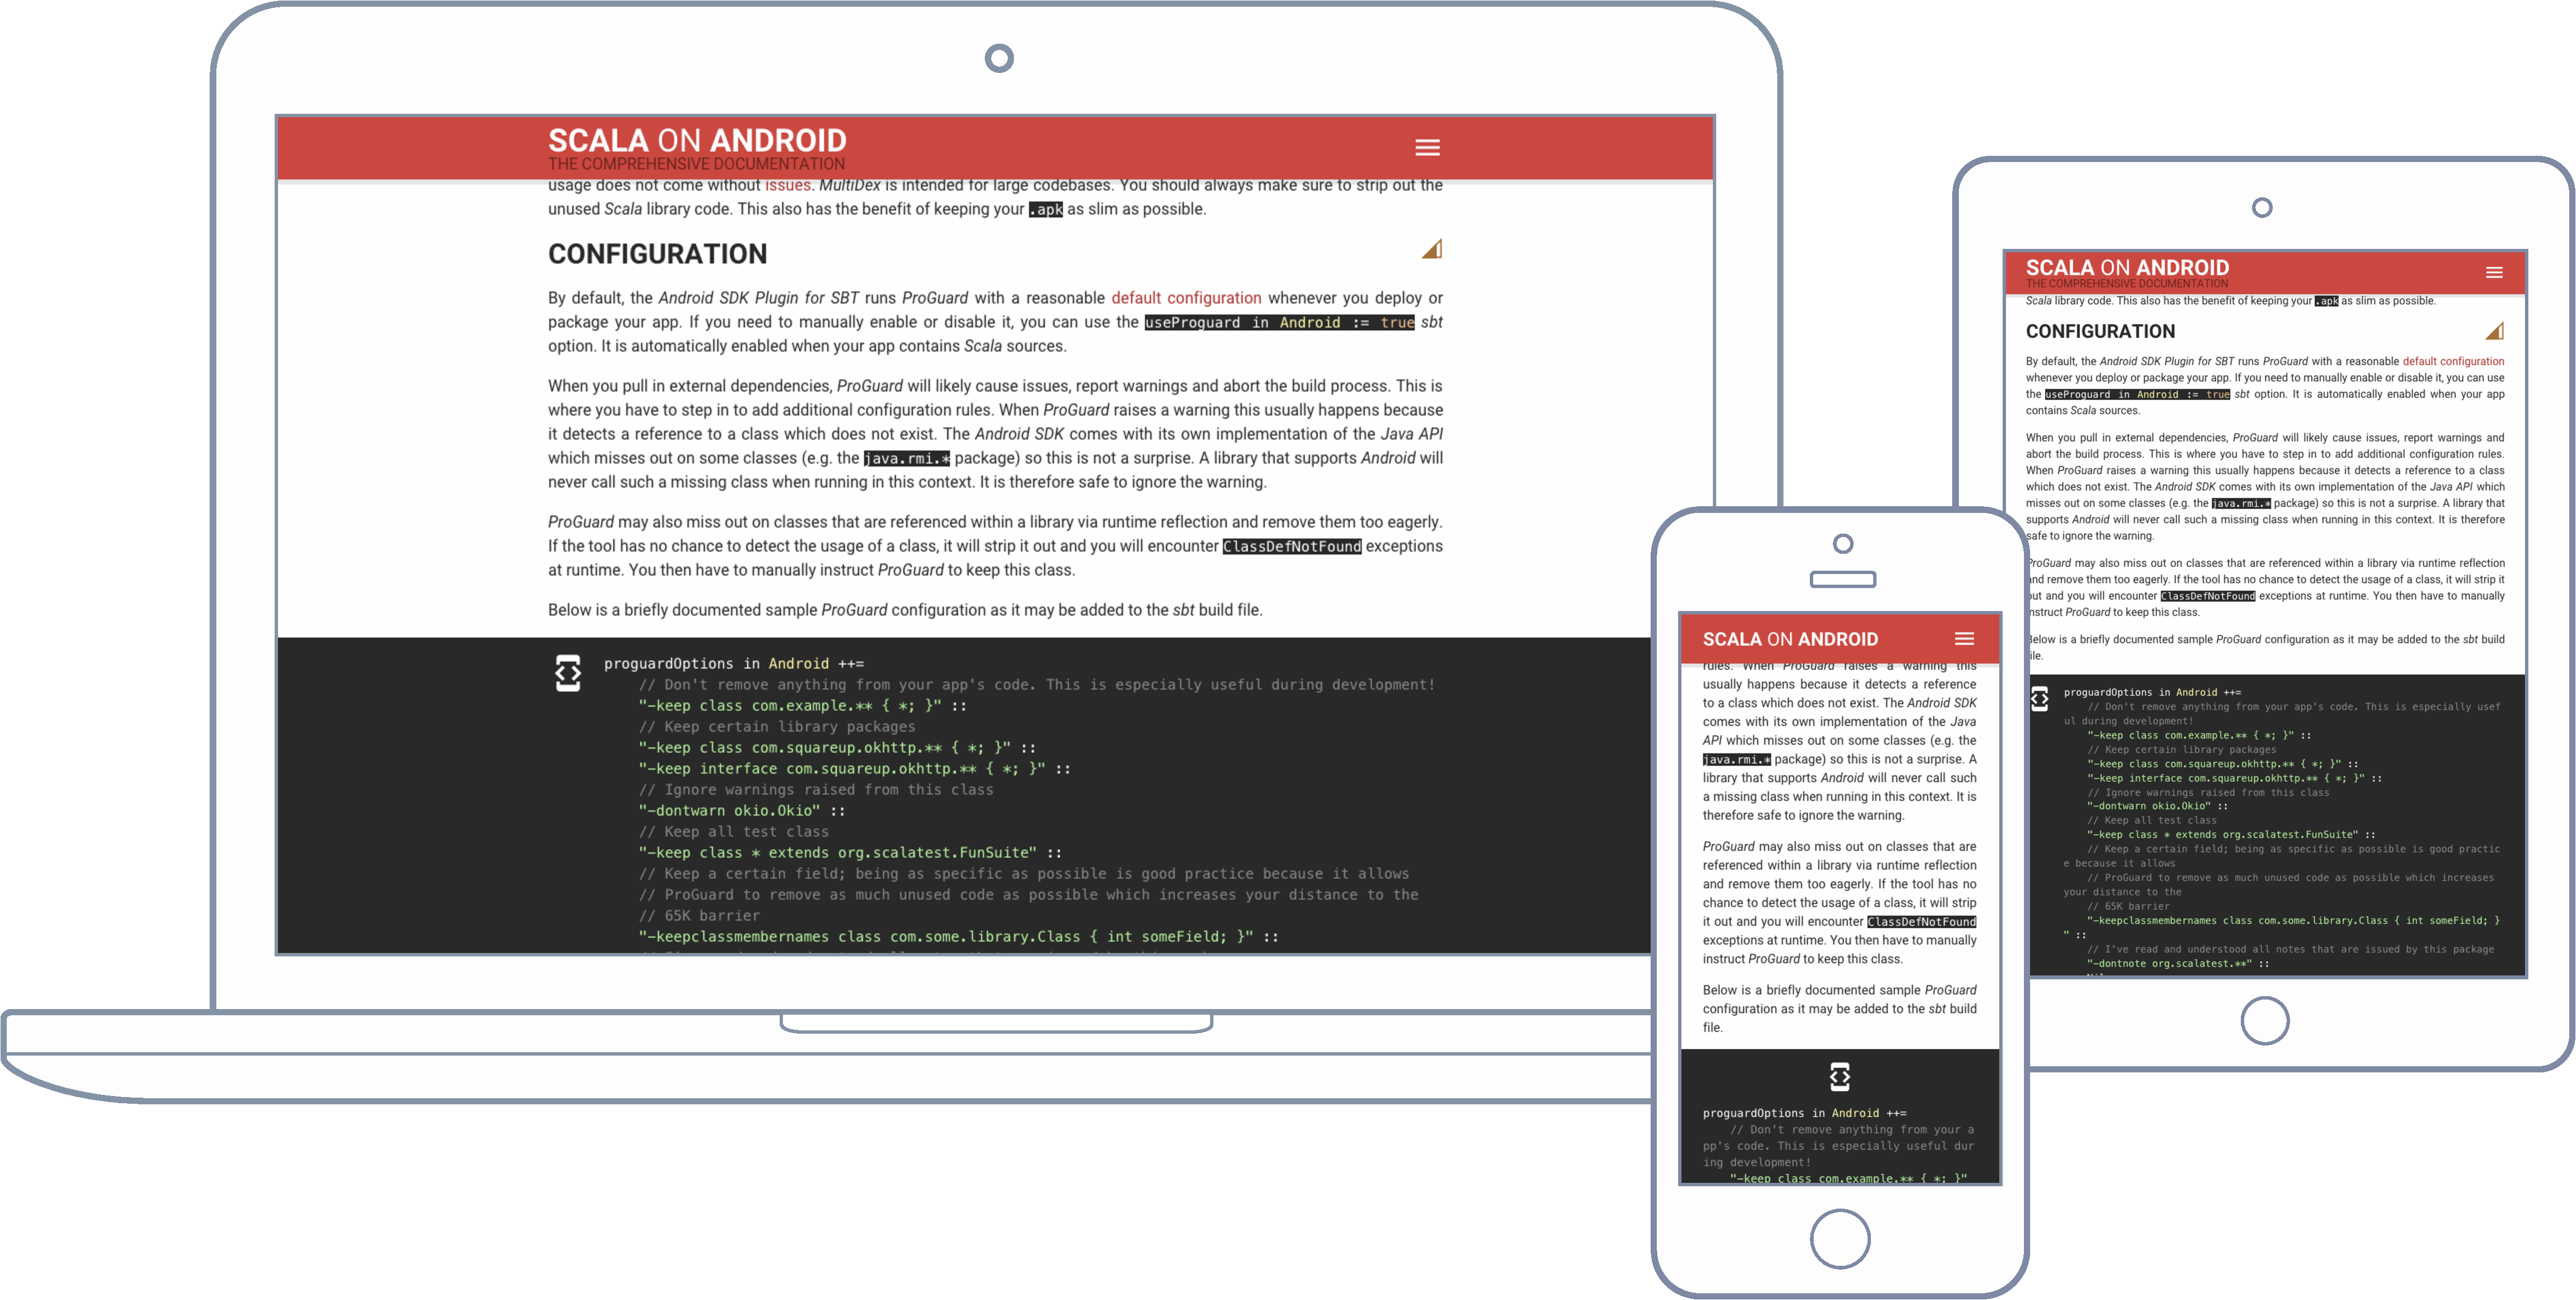
\includegraphics[width=1.5\textwidth]{asset/responsive-design.pdf}}
		\caption{Side by side comparison of the documentation website on common screen sizes}
	\end{figure}

\end{description}